\documentclass[aspectratio=32]{beamer}

\usepackage{beamerthemesplit}
\usetheme{Boadilla}
\usecolortheme{dolphin}
\usefonttheme{serif}

\usepackage{multirow}
\usepackage{subfig}
\usepackage{amssymb,amsmath,mathtools}
\usepackage{amsfonts,booktabs}
\usepackage{lmodern,textcomp}
\usepackage{color}
\usepackage{tikz}
\usetikzlibrary{arrows.meta,calc,positioning,shapes.geometric}
\usepackage{multicol}
\usepackage{graphicx}
\usepackage{ctex}
\usepackage{hyperref}
\usepackage{nicefrac}
\usepackage{tabularx}
\usepackage{ragged2e}

% XeLaTeX 直接处理中文，不需要额外的编码包。
\graphicspath{{material/}}

\setbeamertemplate{navigation symbols}{}
\setbeamertemplate{caption}[numbered]
\setbeamercolor{structure}{fg=blue!70!black}
\setbeamercolor{frametitle}{fg=blue!70!black}
\setbeamerfont{frametitle}{size=\large}
\setlength{\parskip}{2pt}
\setlength{\tabcolsep}{5pt}

\definecolor{LectureBlue}{RGB}{18,18,150}
\definecolor{SoftBlue}{RGB}{235,240,255}
\definecolor{SoftRed}{RGB}{255,239,239}
\definecolor{SoftGreen}{RGB}{235,249,240}
\setbeamercolor{lecturesection}{fg=white,bg=LectureBlue}

\newcommand{\lecturesectionpage}[1]{%
\begin{frame}[plain]
\begin{center}
\vfill
\begin{beamercolorbox}[wd=0.74\textwidth,rounded=true,shadow=true,center,sep=1em]{lecturesection}
\LARGE #1
\end{beamercolorbox}
\vfill
\end{center}
\end{frame}
}

\title[Lecture 1: 课程初衷与内容介绍]{Lecture 1：课程初衷与内容介绍}
\author{陈宠\inst{1}}
\institute{中国人民大学经济学院\inst{1}}
\date{2026年秋季}

\begin{document}

% 1. 封面
\begin{frame}
\maketitle
\end{frame}

% 2. 本讲路线
\begin{frame}{目录}
\tableofcontents[hideallsubsections]
\vspace{0.35cm}
\begin{center}
\textcolor{LectureBlue}{从“为什么学模型”，到“模型怎么讲故事”}
\end{center}
\end{frame}

\section{课程初衷}
\begin{frame}
\begin{center}
    \begin{minipage}{1\textwidth}
	\setbeamercolor{mybox}{fg=white, bg=black!50!blue}
		\begin{beamercolorbox}[wd=0.7\textwidth, rounded=true, shadow=true]{mybox}
			\LARGE \centering 课程初衷
		\end{beamercolorbox}
    \end{minipage}
\end{center} 
\end{frame}


% 3. 为什么不考试
\begin{frame}{课程建立初衷}
\vspace{0.15cm}
\begin{itemize}
    \item 不把“记住定义”当作终点，而是从经济学直觉和朴素判断出发
    \item 数学是表达经济故事的语言：它帮助我们把机制说清楚
    \item 一个好模型不是世界的复制品，而是对问题有用的简化
\end{itemize}
\vspace{0.25cm}
\begin{center}
\begin{center}
\large\textit{All model are wrong, but some are useful.}
\end{center}
\end{center}
\end{frame}


\section{经济学研究范式的变化}
\begin{frame}
\begin{center}
    \begin{minipage}{1\textwidth}
	\setbeamercolor{mybox}{fg=white, bg=black!50!blue}
		\begin{beamercolorbox}[wd=0.70\textwidth, rounded=true, shadow=true]{mybox}
			\LARGE \centering 经济学研究范式的变化
		\end{beamercolorbox}
    \end{minipage}
\end{center} 
\end{frame}

% 6. Atkin and Faber
\begin{frame}{一个切入案例：Atkin and Faber（2026）}
\begin{center}

\includegraphics[width=0.88\textwidth]{atkin_faber_2026_title}
\end{center}
\vspace{-0.05cm}

\begin{center}
\begin{block}{研究问题}
数据和计算能力快速增长之后，国际贸易研究的研究范式发生了什么变化？
\end{block}
\end{center}

\vspace{0.1cm}
\scriptsize\textcolor{gray}{来源：Atkin and Faber (2026), title page, p. 1.}
\end{frame}

% 7. 数据革命的内容
\begin{frame}{现实背景}
\begin{itemize}
    \item \textbf{交易级数据}：企业、产品、订单、价格和交易对手之间的流量；
    \item \textbf{行政数据连接}：将企业、雇员、家庭和地区记录匹配起来；
    \item \textbf{卫星与空间数据}：高分辨率地理影像、夜间灯光、空间距离与网络；
    \item \textbf{计算能力提升}：更高维的状态空间、更复杂的估计与反事实模拟。
\end{itemize}
\begin{block}{Atkin and Faber（2026）}
基于这样的现实背景，经济学研究范式发生了什么变化？
\end{block}
\end{frame}

\begin{frame}{变化一：模型越来越要求匹配现实数据}
\begin{center}
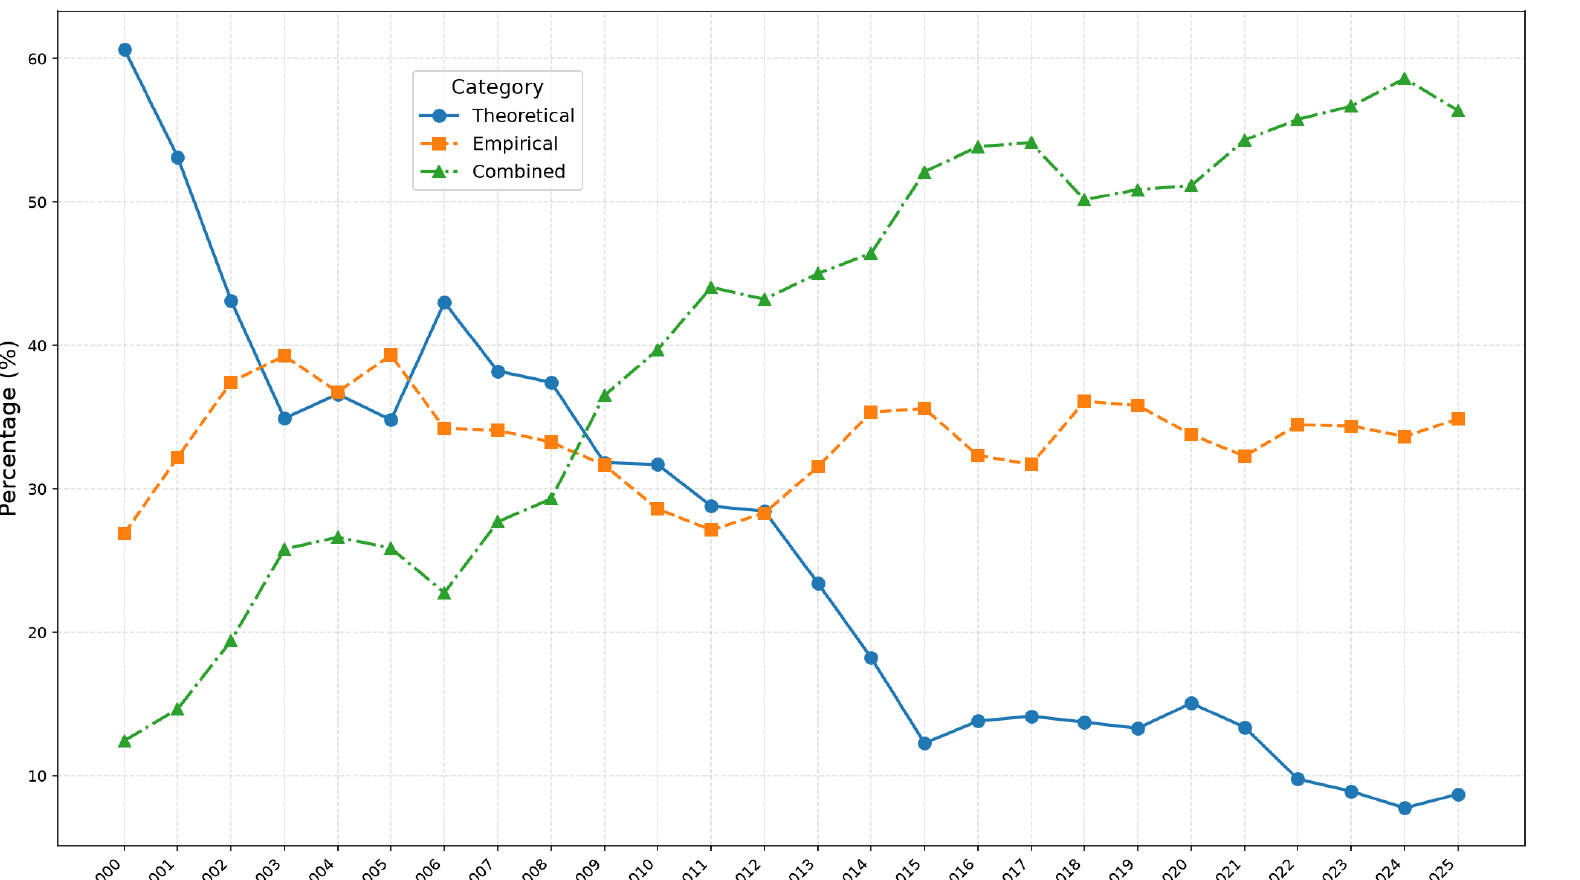
\includegraphics[width=0.83\textwidth,height=5.0cm,keepaspectratio]{atkin_faber_2026_fig1_methodology}
\end{center}
\vspace{-0.04cm}
\begin{columns}[T]
\begin{column}{0.32\textwidth}
\centering\textcolor{LectureBlue}{理论论文}\par
从约 61\% 降至约 9\%
\end{column}
\begin{column}{0.32\textwidth}
\centering\textcolor{orange!85!black}{纯实证}\par
大致稳定在约 30\%--35\%
\end{column}
\begin{column}{0.32\textwidth}
\centering\textcolor{green!50!black}{结合型}\par
从约 12\% 升至约 56\%
\end{column}
\end{columns}
\vspace{0.05cm}
\scriptsize\textcolor{gray}{来源：Atkin and Faber (2026), Figure 1, p. 15；三年移动平均。}
\end{frame}

% 11. Figure 2
\begin{frame}{事实二：结合型研究转向“量化模型与反事实”}
\begin{center}
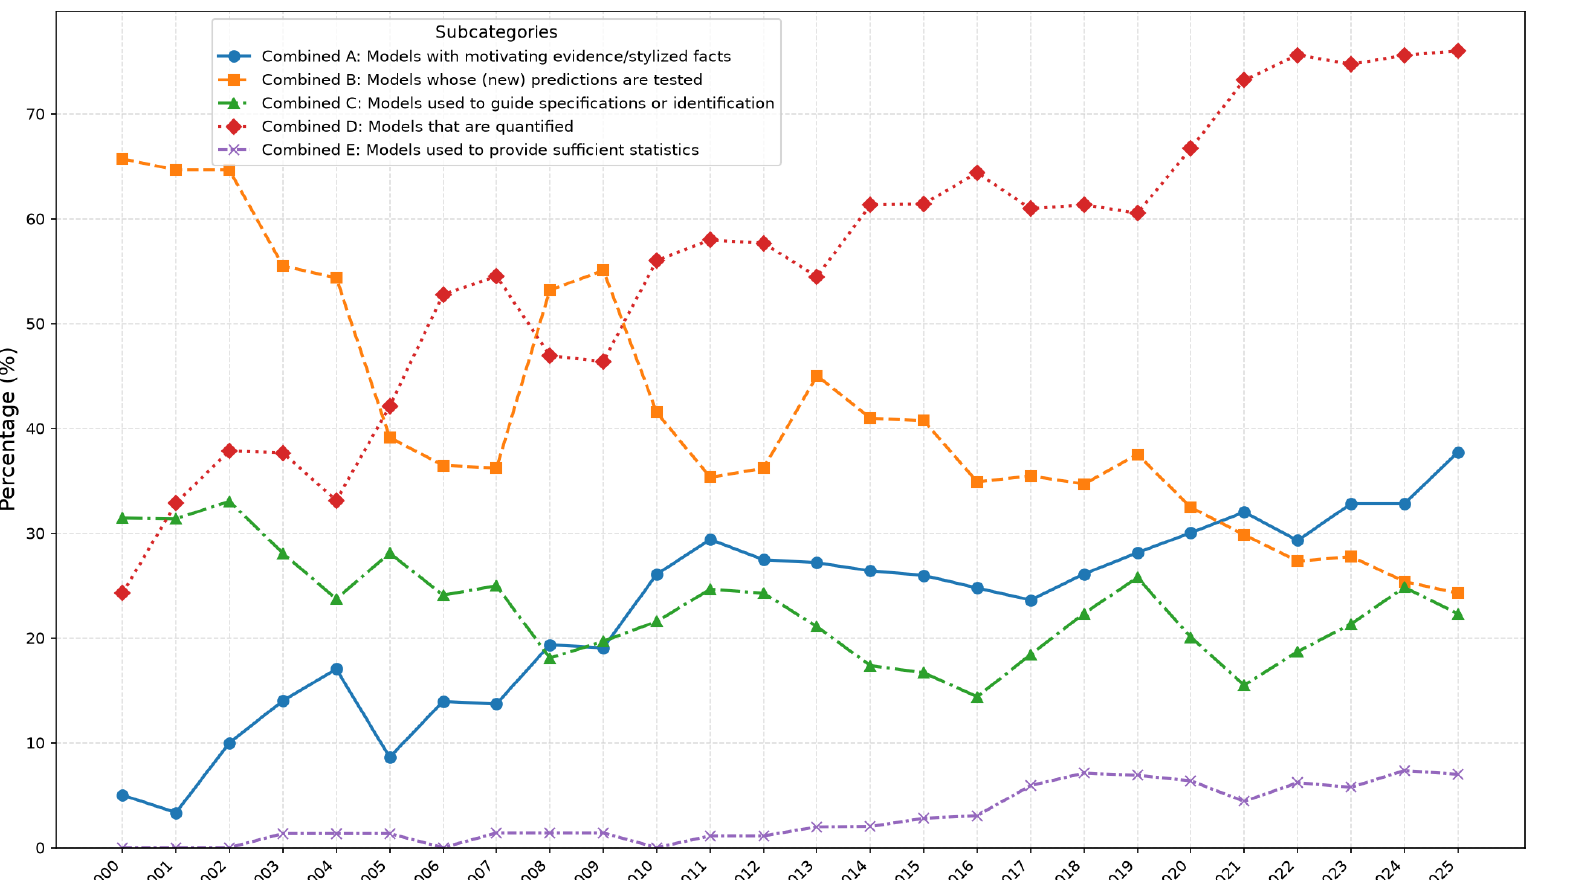
\includegraphics[width=0.83\textwidth,height=4.25cm,keepaspectratio]{atkin_faber_2026_fig2_quantification}
\end{center}
\vspace{-0.04cm}
\begin{itemize}
    \item 早期结合型论文主要是从模型推出预测，再到数据中检验（Combined B）；
    \item 到样本末期，使用数据量化模型、进行反事实分析（Combined D）的比例接近 80\%；
    \item 研究问题由“模型能否解释事实”转向“模型对政策变化有何含义”。
\end{itemize}
\vspace{-0.04cm}
\scriptsize\textcolor{gray}{来源：Atkin and Faber (2026), Figure 2, p. 16；细分类别可多重归类。}
\end{frame}


\section{创新经济学课程路线}
\begin{frame}
\begin{center}
    \begin{minipage}{1\textwidth}
	\setbeamercolor{mybox}{fg=white, bg=black!50!blue}
		\begin{beamercolorbox}[wd=0.7\textwidth, rounded=true, shadow=true]{mybox}
			\LARGE \centering 课程路线图
		\end{beamercolorbox}
    \end{minipage}
\end{center} 
\end{frame}
% 20. 课程路线图
\begin{frame}{课程路线图}
\begin{center}
\begin{tikzpicture}[>=Stealth, every node/.style={font=\small},
    course/.style={draw=LectureBlue, fill=SoftBlue, rounded corners,
        minimum width=3.25cm, minimum height=0.85cm, align=center},
    end/.style={draw=green!50!black, fill=SoftGreen, rounded corners,
        minimum width=3.5cm, minimum height=0.85cm, align=center}]
\node[course] (pf) {生产函数\\投入、产出与 TFP};
\node[course, right=0.38cm of pf] (solow)
    {Solow 模型\\资本积累与增长};
\node[course, right=0.38cm of solow] (romer)
    {Romer / Quality Ladder\\内生创新};

% 源码顺序仍然是 multi → ti → it
\node[end, below=0.72cm of romer] (multi)
    {多部门增长\\生产网络与结构转型};
\node[course, left=0.38cm of multi] (ti)
    {贸易到创新\\市场规模与竞争};
\node[course, left=0.38cm of ti] (it)
    {创新到贸易\\技术与比较优势};

\draw[->, thick] (pf) -- (solow);
\draw[->, thick] (solow) -- (romer);
\draw[->, thick] (romer) -- (it);
\draw[->, thick] (it) -- (ti);
\draw[->, thick] (ti) -- (multi);
\end{tikzpicture}
\end{center}
\end{frame}


% 22. 参考文献与结尾
\begin{frame}{参考文献}
\small
\begin{thebibliography}{9}
\bibitem{atkinfaber}
Atkin, D. and B. Faber (2026). \newblock \emph{The Data Revolution, and Its Uses, in International Trade}. August 2026.
\end{thebibliography}
\vfill

\begin{center}
\makebox[\textwidth][c]{%
\begin{beamercolorbox}[
    wd=0.70\textwidth,
    rounded=true,
    shadow=true,
    center,
    sep=0.8em
]{lecturesection}
    \centering
    \Huge Thanks!\\[0.25cm]
    \large\texttt{chenchong@ruc.edu.cn}
\end{beamercolorbox}%
}
\end{center}
\end{frame}

\end{document}
